\documentclass[11pt,a4paper]{article}

\usepackage[utf8]{inputenc}
\usepackage[T1]{fontenc}
\usepackage{lmodern}
\usepackage[spanish,es-tabla,es-nodecimaldot]{babel}
\usepackage{geometry}
\geometry{margin=2.5cm}
\usepackage{graphicx}
\usepackage{booktabs}
\usepackage{array}
\usepackage{needspace}
\usepackage{amsmath,amssymb,amsthm}
\usepackage{enumitem}
\usepackage{listings}
\usepackage{xcolor}
\usepackage{float}
\usepackage{tikz}
\usepackage{pgfplots}
\pgfplotsset{compat=1.18}
\usepackage{caption}
\usepackage{subcaption}
\usepackage[colorlinks=true,urlcolor=blue!60!black,linkcolor=black,citecolor=black]{hyperref}

\definecolor{cquery}{HTML}{F39C12}
\definecolor{clca}{HTML}{2ECC71}
\definecolor{cedge}{HTML}{D4A20B}

\lstset{
  basicstyle=\ttfamily\footnotesize,
  frame=single,
  breaklines=true,
  columns=fullflexible,
  keywordstyle=\color{blue!60!black}\bfseries,
  commentstyle=\color{gray}\itshape,
  language=C++,
  literate={á}{{\'a}}1 {é}{{\'e}}1 {í}{{\'i}}1 {ó}{{\'o}}1 {ú}{{\'u}}1 {ñ}{{\~n}}1
}

\theoremstyle{plain}
\newtheorem{lema}{Lema}
\newtheorem{prop}{Proposición}

% ---------- DATOS DEL GRUPO ----------
\newcommand{\IntegranteA}{Gabriel Murillo Machicao}
\newcommand{\IntegranteB}{Juan Pablo Saavedra Ruiz}
% -------------------------------------

\emergencystretch=2em

\begin{document}

% ======================= CARÁTULA =======================
\begin{titlepage}
  \centering
  \vspace*{2cm}
  {\Large \textbf{Universidad de Ingeniería y Tecnología (UTEC)}\par}
  {\large Ciencia de la Computación\par}
  \vspace{2cm}
  {\Huge \textbf{Proyecto Final 2}\par}
  \vspace{0.4cm}
  {\Large Anima tu Algoritmo o Estructura de Datos\par}
  \vspace{1.5cm}
  {\large CS2023 -- Algoritmos y Estructuras de Datos (2026-2)\par}
  {\large Profesor: Wilder Nina Choquehuayta\par}
  \vspace{2cm}
  {\Large Estructura asignada:\par}
  {\Huge \textbf{Virtual Tree (Auxiliary Tree)}\par}
  \vspace{2cm}
  {\large \textbf{Integrantes}\par}
  \vspace{0.3cm}
  {\large \IntegranteA\par}
  {\large \IntegranteB\par}
  \vfill
  {\large Lima, noviembre de 2026\par}
\end{titlepage}

\tableofcontents
\newpage

% ======================= 1. DESCRIPCIÓN =======================
\section{Descripción de la estructura y su TDA}

Un \emph{Virtual Tree} (o \emph{Auxiliary Tree}) es un árbol construido a partir de un
subconjunto $S$ de $k$ nodos de un árbol enraizado $T$ de $n$ nodos. Contiene los nodos de
$S$ y, además, los ancestros comunes más bajos (LCA) necesarios para preservar las relaciones
de ancestro entre ellos. Cada arista $(p, v)$ del virtual tree representa un camino
$p \rightsquigarrow v$ de $T$ cuyos nodos intermedios no pertenecen a la estructura, de modo
que el resultado tiene a lo sumo $2k-1$ nodos, independientemente de $n$.

\paragraph{TDA que representa.} Dado un árbol enraizado fijo $T$ (que se preprocesa una
sola vez), la estructura ofrece las operaciones:
\begin{center}
\begin{tabular}{@{}ll@{}}
  \toprule
  \textbf{Operación} & \textbf{Descripción} \\
  \midrule
  \textsc{Preprocesar}$(T)$ & calcula \texttt{tin}, \texttt{tout}, profundidades y la estructura de LCA \\
  \textsc{EsAncestro}$(u, v)$ & ¿$u$ es ancestro de $v$? en $O(1)$ \\
  \textsc{LCA}$(u, v)$ & ancestro común más bajo de $u$ y $v$, en $O(1)$ \\
  \textsc{Virtual}$(S) \to (V', E')$ & devuelve el árbol comprimido sobre $S$ \\
  \bottomrule
\end{tabular}
\end{center}

\paragraph{Definición formal.} Sea $V' = \operatorname{cl}_{\mathrm{LCA}}(S)$ la clausura de
$S$ bajo la operación LCA (el menor conjunto que contiene a $S$ y a $\mathrm{lca}(a,b)$ para
todo par $a, b$ del conjunto). Para cada $v \in V'$ distinto de la raíz de $V'$, su
\emph{padre virtual} es el ancestro propio más cercano de $v$ que pertenece a $V'$; las
aristas $E'$ son los pares (padre virtual, $v$).

\paragraph{¿Para qué sirve?} Su uso típico es la programación dinámica sobre árboles con
muchas consultas, donde cada consulta solo involucra $k$ nodos relevantes y la suma de los
$k$ está acotada. Resolver cada consulta con un DFS sobre todo $T$ cuesta $O(n)$ por
consulta; sobre el virtual tree cuesta $O(k \log k)$. Un ejemplo clásico es el problema
\emph{Kingdom and Its Cities} (Codeforces 613D).

\begin{figure}[H]
  \centering
  \begin{tikzpicture}[
      every node/.style={circle, draw=black!70, minimum size=6.5mm, inner sep=0pt, font=\small},
      q/.style={fill=cquery!80},
      l/.style={fill=clca!70},
      b/.style={fill=black!8},
      tl/.style={draw=none, fill=none, font=\scriptsize\color{black!60}, minimum size=0pt},
      x=0.95cm, y=1.05cm]
    % árbol original
    \node[l] (0) at (2.75,0) {0};
    \node[l] (1) at (1.25,-1) {1};   \node[l] (2) at (4.25,-1) {2};
    \node[b] (3) at (0.5,-2) {3};    \node[b] (4) at (2,-2) {4};
    \node[b] (5) at (3.5,-2) {5};    \node[b] (6) at (5,-2) {6};
    \node[q] (7) at (0,-3) {7};      \node[b] (8) at (1,-3) {8};
    \node[q] (9) at (2,-3) {9};      \node[q] (10) at (3,-3) {10};
    \node[b] (11) at (4,-3) {11};    \node[b] (12) at (5,-3) {12};
    \node[q] (13) at (5,-4) {13};
    \foreach \a/\b in {0/1,0/2,1/3,1/4,2/5,2/6,3/7,3/8,4/9,5/10,5/11,6/12,12/13}
      \draw (\a) -- (\b);
    \foreach \v/\t in {0/0,1/1,2/7,3/2,4/5,5/8,6/11,7/3,8/4,9/6,10/9,11/10,12/12,13/13}
      \node[tl, anchor=west] at ([xshift=0.5pt]\v.east) {\t};
    \node[draw=none, font=\small] at (2.5,-4.9) {(a) Árbol $T$ ($n = 14$); en gris, \texttt{tin}.};

    % virtual tree
    \begin{scope}[xshift=8.3cm]
      \node[l] (v0) at (1.5,0) {0};
      \node[l] (v1) at (0.5,-1.5) {1};  \node[l] (v2) at (2.5,-1.5) {2};
      \node[q] (v7) at (0,-3) {7};      \node[q] (v9) at (1,-3) {9};
      \node[q] (v10) at (2,-3) {10};    \node[q] (v13) at (3,-3) {13};
      \foreach \a/\b in {v0/v1,v0/v2,v1/v7,v1/v9,v2/v10,v2/v13}
        \draw[cedge, line width=1.6pt] (\a) -- (\b);
      \node[draw=none, font=\small] at (1.5,-4.9) {(b) Virtual tree de $S=\{10,7,13,9\}$.};
    \end{scope}
  \end{tikzpicture}
  \caption{Ejemplo usado en el video. En naranja, los nodos de la consulta; en verde, los
  LCA añadidos. La arista $(2, 13)$ comprime el camino $2 \to 6 \to 12 \to 13$.}
  \label{fig:ejemplo}
\end{figure}

% ======================= 2. ALGORITMO =======================
\section{Algoritmo implementado}

La implementación (\texttt{cpp/virtual\_tree.hpp}) es propia y no usa librerías de terceros
que implementen la estructura. Consta de un preprocesamiento sobre $T$ y de dos variantes de
construcción.

\subsection{Preprocesamiento}
\begin{itemize}
  \item \textbf{DFS iterativo} con pila explícita que calcula, para cada nodo, el tiempo de
        entrada \texttt{tin}, el de salida \texttt{tout}, su profundidad y su padre. Con ellos,
        $\textsc{EsAncestro}(u,v) \iff \mathtt{tin}[u] \le \mathtt{tin}[v] \le \mathtt{tout}[u]$
        se decide en $O(1)$. Se usa la versión iterativa (en lugar de la recursiva) para no
        desbordar la pila del sistema en árboles muy profundos: las pruebas incluyen una cadena
        de $10^6$ nodos.
  \item \textbf{Euler tour + Sparse Table}: el LCA de $u$ y $v$ es el nodo de menor
        profundidad entre sus primeras apariciones en el recorrido de Euler, lo que se
        responde en $O(1)$ con una Sparse Table de $O(n \log n)$.
\end{itemize}

\subsection{\texorpdfstring{Construcción general: \texttt{build\_virtual} ($O(k \log k)$)}{Construcción general: build\_virtual, O(k log k)}}
Acepta la consulta en cualquier orden y con duplicados. Es la variante que se anima en el video.
\begin{enumerate}[label=\textbf{\arabic*.}]
  \item \textbf{Ordenar} los nodos de la consulta por \texttt{tin} y eliminar duplicados.
  \item \textbf{Añadir LCAs}: agregar $\mathrm{lca}(s_i, s_{i+1})$ para cada par de nodos
        adyacentes en ese orden; ordenar de nuevo por \texttt{tin} y eliminar duplicados.
  \item \textbf{Pila}: recorrer los nodos en orden de \texttt{tin}; sacar de la pila los
        nodos que no son ancestros del nodo actual; si la pila queda no vacía, su tope es el
        padre virtual y se agrega la arista; finalmente, apilar el nodo actual.
\end{enumerate}

\begin{lstlisting}
for (int v : all) {                       // all: consulta + LCAs, ordenados por tin
    while (!st.empty() && !is_ancestor(st.back(), v)) st.pop_back();
    if (!st.empty()) edges.push_back({st.back(), v});   // padre virtual = tope
    st.push_back(v);
}
\end{lstlisting}

\subsection{Correctitud}

\begin{lema}\label{lem:adyacentes}
Sea $s_1, \dots, s_k$ la consulta ordenada por \texttt{tin}. Para todo $i < j$,
$\mathrm{lca}(s_i, s_j)$ es igual a $\mathrm{lca}(s_t, s_{t+1})$ para algún $t \in [i, j-1]$;
en concreto, al de menor profundidad entre ellos.
\end{lema}
\begin{proof}[Idea de la prueba]
Sea $w = \mathrm{lca}(s_i, s_j)$. Como $s_i$ y $s_j$ están en el subárbol de $w$ y el
subárbol de $w$ ocupa un intervalo contiguo de \texttt{tin}, todos los $s_t$ con
$i \le t \le j$ también están en él; luego cada $\mathrm{lca}(s_t, s_{t+1})$ es descendiente
(o igual) de $w$. Por otro lado, $s_i$ y $s_j$ están en subárboles de hijos distintos de $w$
(o uno de ellos es $w$), así que existe un $t$ en el que la secuencia «salta» de un hijo a
otro, y para ese $t$ se cumple $\mathrm{lca}(s_t, s_{t+1}) = w$.
\end{proof}

\begin{prop}
$V' = S \cup \{\mathrm{lca}(s_t, s_{t+1}) : 1 \le t < k\}$, y por tanto
$|V'| \le k + (k-1) = 2k-1$.
\end{prop}
Esto justifica el paso 2: bastan $k-1$ consultas de LCA (en vez de las $\binom{k}{2}$ de todos
los pares) y el árbol resultante nunca supera $2k-1$ nodos.

\paragraph{Invariante de la pila.} Al procesar los nodos de $V'$ en orden de \texttt{tin},
la pila contiene, de la base al tope, la cadena de ancestros (en $V'$) del último nodo
procesado. Cuando llega $v$, todos sus ancestros en $V'$ ya fueron procesados (tienen menor
\texttt{tin}) y siguen en la pila, mientras que los nodos que se sacan no son ancestros de
$v$ ni de ningún nodo posterior. Por eso, tras sacar los no-ancestros, el tope es exactamente
el ancestro propio más cercano de $v$ en $V'$, es decir, su padre virtual.

\subsection{Traza del ejemplo}
La tabla~\ref{tab:traza} reproduce la traza real que genera el programa \texttt{cpp/trace\_gen.cpp} para
la consulta $[10, 7, 13, 9]$ de la figura~\ref{fig:ejemplo}. Ordenada por \texttt{tin} queda
$[7, 9, 10, 13]$; los LCA de pares adyacentes son $\mathrm{lca}(7,9)=1$,
$\mathrm{lca}(9,10)=0$ y $\mathrm{lca}(10,13)=2$; tras la segunda ordenación se recorre
$[0, 1, 7, 9, 2, 10, 13]$.

\begin{table}[H]
  \centering
  \begin{tabular}{@{}cccccc@{}}
    \toprule
    \textbf{Paso} & \textbf{Nodo} & \textbf{Se sacan} & \textbf{Padre virtual} &
    \textbf{Arista} & \textbf{Pila (base $\to$ tope)} \\
    \midrule
    1 & 0  & ---      & --- (raíz) & ---       & $[0]$ \\
    2 & 1  & ---      & 0          & $(0,1)$   & $[0, 1]$ \\
    3 & 7  & ---      & 1          & $(1,7)$   & $[0, 1, 7]$ \\
    4 & 9  & 7        & 1          & $(1,9)$   & $[0, 1, 9]$ \\
    5 & 2  & 9, 1     & 0          & $(0,2)$   & $[0, 2]$ \\
    6 & 10 & ---      & 2          & $(2,10)$  & $[0, 2, 10]$ \\
    7 & 13 & 10       & 2          & $(2,13)$  & $[0, 2, 13]$ \\
    \bottomrule
  \end{tabular}
  \caption{Pasos de la pila para la consulta $[10, 7, 13, 9]$: 7 nodos y 6 aristas
  (cota $2k-1 = 7$).}
  \label{tab:traza}
\end{table}

\subsection{\texorpdfstring{Variante con entrada ordenada: \texttt{build\_virtual\_sorted} ($O(k)$)}{Variante con entrada ordenada: build\_virtual\_sorted, O(k)}}
Si la consulta ya viene ordenada por \texttt{tin} y sin duplicados (por ejemplo, porque el
problema la entrega así o porque se ordenó una vez y se reutiliza), no es necesario ordenar
dos veces: el LCA se inserta en el momento en que se necesita, en una sola pasada.

\begin{lstlisting}
st = {q[0]};
for (i = 1; i < k; ++i) {
    v = q[i];  l = lca(st.back(), v);
    if (l != st.back()) {                       // v sale del subárbol del tope
        while (st.size() >= 2 && depth[st[st.size()-2]] >= depth[l]) {
            edges.push_back({st[st.size()-2], st.back()});  st.pop_back();
        }
        if (st.back() != l) {                   // l es un punto de ramificación nuevo
            edges.push_back({l, st.back()});  st.pop_back();  st.push_back(l);
        }
    }
    st.push_back(v);
}
// al final se unen los nodos que quedan en la pila, de tope a base
\end{lstlisting}

Cada nodo entra y sale de la pila una vez y se hacen $k-1$ consultas de LCA en $O(1)$, por lo
que la construcción es $O(k)$.

\subsection{Casos borde considerados}
\begin{itemize}
  \item \textbf{Consulta vacía}: el resultado es vacío (ambas variantes).
  \item \textbf{$k=1$}: el virtual tree es un único nodo, sin aristas.
  \item \textbf{Un nodo de la consulta es ancestro de otro}: no se añaden LCA nuevos y las
        aristas comprimen los caminos intermedios (en el video, $[2, 6, 13]$ produce
        $2 \to 6 \to 13$, omitiendo el nodo 12).
  \item \textbf{Elementos repetidos} en la consulta: se eliminan tras ordenar.
  \item \textbf{Árboles muy profundos}: el DFS iterativo procesa una cadena de $10^6$ nodos
        sin desbordar la pila.
\end{itemize}

\subsection{Verificación}
\texttt{cpp/tests.cpp} compara ambas variantes con una implementación por fuerza bruta de la
definición formal (clausura bajo LCA de todos los pares y padre virtual subiendo por el árbol)
en 3000 árboles y consultas aleatorias (con duplicados). Para cada caso se comprueba que los
nodos y aristas coinciden, que no hay nodos repetidos, que $|V'| \le 2k-1$ y que
$|E'| = |V'| - 1$. Además se prueban la consulta vacía y la cadena de $10^6$ nodos. Todas las
pruebas pasan (\texttt{make test}).

% ======================= 3. HERRAMIENTAS =======================
\section{Herramientas usadas y pasos para reproducir el video}

\begin{table}[H]
  \centering
  \begin{tabular}{@{}>{\raggedright\arraybackslash}p{5.6cm}p{8.6cm}@{}}
    \toprule
    \textbf{Herramienta} & \textbf{Uso} \\
    \midrule
    C++17 (\texttt{g++} 13.3) & implementación, pruebas, benchmark y generador de traza \\
    Python 3.13 + Manim Community 0.22.1 & renderizado de la animación \\
    Cairo, Pango y FFmpeg 6.1 & dependencias del sistema de Manim \\
    \LaTeX{} (TikZ, pgfplots) & este informe y sus figuras \\
    \bottomrule
  \end{tabular}
\end{table}

\subsection*{Animación impulsada por la implementación real}
\texttt{cpp/trace\_gen.cpp} ejecuta \texttt{build\_virtual} sobre el árbol de la
figura~\ref{fig:ejemplo} y escribe \texttt{manim/trace.json} con los tiempos de entrada, los
LCA y cada paso de la pila. La escena de Manim, \texttt{manim/virtual\_tree\_scene.py},
solo lee ese archivo y lo dibuja; ningún paso del algoritmo está escrito a mano. Así, lo que se
explica en el video es exactamente lo que hace el código.

\subsection*{Estructura del video (1080p60, 4 min 50 s, sin narración)}
El guion está pensado para alguien que ve la estructura por primera vez: primero se plantea
una pregunta concreta y se muestra la meta, luego las dos herramientas que usa el algoritmo
y, recién después, el algoritmo paso a paso.
\begin{enumerate}[label=\arabic*.]
  \item \textbf{El problema}: un árbol grande, una consulta de 4 nodos y la pregunta
        «¿cuántas aristas tiene el menor subárbol que une los nodos marcados?». El árbol se
        comprime en pantalla hasta el virtual tree (la meta antes del método).
  \item \textbf{¿Qué es? (TDA)}: entrada, salida y cota $2k-1$.
  \item \textbf{Herramienta 1, \texttt{tin}/\texttt{tout}}: un punto recorre el árbol siguiendo
        el Euler tour real y numera cada nodo al entrar; cada subárbol aparece como un bloque
        contiguo del arreglo. Se muestra la prueba de ancestro con un ejemplo y luego se
        \emph{pregunta} al espectador otro caso, con cuenta regresiva antes de la respuesta.
  \item \textbf{Herramienta 2, LCA}: los dos caminos que suben hasta encontrarse.
  \item \textbf{El algoritmo en 3 pasos} (hoja de ruta).
  \item \textbf{Ejemplo completo ($k=4$)}: una columna fija indica el paso actual y la leyenda
        de colores. Los nodos de la consulta viajan a su posición ordenada; para cada par vecino
        se dibuja el camino hasta su LCA. En la pila, los nodos apilados llevan un anillo dorado
        en el árbol (se \emph{ve} que la pila es siempre un camino desde la raíz); cada salida
        se justifica con la prueba de intervalos y se explica por qué es seguro sacar un nodo.
        Al final se responde la pregunta inicial sumando la longitud de cada arista virtual:
        $1+2+2+1+2+3 = 11$ aristas, usando solo 7 nodos.
  \item \textbf{¿Por qué bastan los pares vecinos?}: demostración visual. Se pintan los
        subárboles de 1 y de 2; al recorrer la consulta por \texttt{tin} el color cambia una
        sola vez, justo entre dos vecinos, cuyo LCA ya se calculó.
  \item \textbf{Caso borde}: un nodo de la consulta es ancestro de otro (y el caso $k=1$).
  \item \textbf{Tu turno}: ejercicio con pista y cuenta regresiva; solución y respuesta a la
        misma pregunta ($3+1+2+2 = 8$ aristas).
  \item \textbf{¿Cuánto cuesta?}: complejidad y un gráfico de barras con la medición real
        de \texttt{make bench}.
  \item \textbf{Resumen} y créditos.
\end{enumerate}

\subsection*{Criterios didácticos y cómo se verificaron}
Como el video no tiene voz, todo se explica con animación y subtítulos. Se impusieron tres
reglas y se verificaron automáticamente sobre el video renderizado:
\begin{itemize}
  \item \textbf{Tiempo de lectura}: cada subtítulo permanece en pantalla al menos
        $0.6 + \text{caracteres}/15$ segundos (mínimo 1.8~s). La escena lo garantiza esperando
        lo necesario antes de cambiar el texto y registra cada subtítulo con su tiempo;
        un script comprueba que ninguno quede por debajo.
  \item \textbf{Nada fuera de cuadro}: se revisan todos los fotogramas (2 por segundo) en
        busca de contenido que toque los bordes.
  \item \textbf{Duración máxima de 5 minutos.}
\end{itemize}

\subsection*{Pasos para reproducir}
\begin{lstlisting}[language=bash]
cd virtual-tree-animation    # carpeta del proyecto
sudo apt install libcairo2-dev libpango1.0-dev ffmpeg   # Ubuntu/Debian
pip install manim
make test      # pruebas en C++
make bench     # mediciones de tiempo
make video     # genera trace.json y renderiza el .mp4 (1080p60)
make informe   # compila este informe
\end{lstlisting}
El video queda en
\path{manim/media/videos/virtual_tree_scene/1080p60/VirtualTreeVideo.mp4}.

% ======================= 4. CONTRIBUCIONES =======================
\section{Contribuciones de cada integrante}

\begin{table}[H]
  \centering
  \begin{tabular}{@{}>{\raggedright\arraybackslash}p{4.4cm}p{10.1cm}@{}}
    \toprule
    \textbf{Integrante} & \textbf{Contribución} \\
    \midrule
    \IntegranteA & Implementación en C++ (\texttt{virtual\_tree.hpp}: preprocesamiento, LCA
      con Sparse Table, ambas variantes de construcción), pruebas contra fuerza bruta y
      benchmark. \\
    \IntegranteB & Generador de traza, escena de Manim, guion y renderizado del video,
      figuras del informe. \\
    Ambos & Análisis de complejidad y de correctitud, redacción del informe y del README,
      revisión del video. \\
    \bottomrule
  \end{tabular}
\end{table}

% ======================= 5. COMPLEJIDAD =======================
\Needspace{18\baselineskip}
\section{Análisis de complejidad}

Sea $n$ el tamaño del árbol original y $k$ el tamaño de la consulta.

\begin{table}[H]
  \centering
  \begin{tabular}{@{}p{7.6cm}ll@{}}
    \toprule
    \textbf{Paso} & \textbf{Tiempo} & \textbf{Espacio} \\
    \midrule
    DFS iterativo (\texttt{tin}, \texttt{tout}, profundidad) & $O(n)$ & $O(n)$ \\
    Euler tour + Sparse Table & $O(n \log n)$ & $O(n \log n)$ \\
    Consulta \textsc{LCA} / \textsc{EsAncestro} & $O(1)$ & --- \\
    \midrule
    \multicolumn{3}{@{}l}{\textit{\texttt{build\_virtual} (entrada arbitraria)}} \\
    Ordenar $k$ nodos por \texttt{tin} & $O(k \log k)$ & $O(k)$ \\
    $k-1$ LCAs y segunda ordenación ($\le 2k-1$ nodos) & $O(k \log k)$ & $O(k)$ \\
    Construcción con pila & $O(k)$ & $O(k)$ \\
    \textbf{Total por consulta} & $\boldsymbol{O(k \log k)}$ & $O(k)$ \\
    \midrule
    \multicolumn{3}{@{}l}{\textit{\texttt{build\_virtual\_sorted} (entrada ordenada por \texttt{tin})}} \\
    \textbf{Total por consulta} & $\boldsymbol{O(k)}$ & $O(k)$ \\
    \bottomrule
  \end{tabular}
\end{table}

\noindent En la fase de pila cada nodo entra y sale a lo sumo una vez, de modo que es lineal.
El preprocesamiento se paga una sola vez y se amortiza entre todas las consultas: con $q$
consultas cuya suma de tamaños es $K$, el costo total es $O(n \log n + K \log K)$, frente a
$O(n \cdot q)$ si se recorriera el árbol completo en cada consulta.

\subsection{Resultados empíricos}
\texttt{cpp/bench.cpp} mide el tiempo promedio por consulta sobre árboles aleatorios
(compilado con \texttt{-O2}; máquina virtual Intel Xeon a 2.1~GHz; los valores absolutos
dependen del equipo, lo relevante es cómo crecen).

\begin{table}[H]
  \centering
  \begin{subtable}[t]{0.47\textwidth}
    \centering
    \begin{tabular}{@{}rrr@{}}
      \toprule
      $n$ & \texttt{build\_virtual} & recorrido $O(n)$ \\
      \midrule
      $10^3$ & 17.5~µs & 0.6~µs \\
      $10^4$ & 17.7~µs & 6.9~µs \\
      $10^5$ & 21.2~µs & 151.6~µs \\
      $10^6$ & 35.1~µs & 1563.7~µs \\
      \bottomrule
    \end{tabular}
    \caption{$k = 100$ fijo, $n$ variable.}
  \end{subtable}\hfill
  \begin{subtable}[t]{0.5\textwidth}
    \centering
    \begin{tabular}{@{}rrrr@{}}
      \toprule
      $k$ & general & ordenada & $|V'|$ prom. \\
      \midrule
      $10$     & 3.2~µs   & 2.1~µs  & 15.7 \\
      $10^2$   & 34.3~µs  & 12.4~µs & 164.2 \\
      $10^3$   & 0.40~ms  & 0.10~ms & 1\,634 \\
      $10^4$   & 3.86~ms  & 0.89~ms & 15\,959 \\
      $10^5$   & 46.1~ms  & 8.10~ms & 137\,966 \\
      \bottomrule
    \end{tabular}
    \caption{$n = 10^6$ fijo, $k$ variable.}
  \end{subtable}
  \caption{Tiempo promedio por consulta.}
  \label{tab:bench}
\end{table}

\begin{figure}[H]
  \centering
  \begin{tikzpicture}
    \begin{loglogaxis}[
        width=0.72\textwidth, height=6cm,
        xlabel={$k$ (tamaño de la consulta)}, ylabel={tiempo por consulta (µs)},
        legend pos=north west, legend cell align=left, grid=major,
        grid style={black!12}]
      \addplot[mark=*, color=cquery!90!black, thick]
        coordinates {(10,3.16) (100,34.34) (1000,398.57) (10000,3858.54) (100000,46108.67)};
      \addlegendentry{\texttt{build\_virtual} ($O(k\log k)$)}
      \addplot[mark=square*, color=clca!70!black, thick]
        coordinates {(10,2.06) (100,12.37) (1000,99.41) (10000,889.32) (100000,8099.93)};
      \addlegendentry{\texttt{build\_virtual\_sorted} ($O(k)$)}
      \addplot[dashed, black!60, domain=10:100000, samples=2] {1563.74};
      \addlegendentry{recorrer todo el árbol ($n=10^6$)}
    \end{loglogaxis}
  \end{tikzpicture}
  \caption{Tiempo por consulta en función de $k$ con $n = 10^6$ (escala log-log).}
  \label{fig:bench}
\end{figure}

\paragraph{Lectura de los resultados.}
\begin{itemize}
  \item Con $k$ fijo, multiplicar $n$ por 1000 apenas duplica el tiempo de
        \texttt{build\_virtual} (de 17.5 a 35.1~µs), mientras que el recorrido completo crece
        de forma lineal. El leve aumento no se debe al algoritmo, sino a que con $n$ grande
        los arreglos \texttt{tin} y la Sparse Table ya no caben en caché y cada acceso
        aleatorio es más lento.
  \item Con $n$ fijo, el tiempo de \texttt{build\_virtual} crece algo más rápido que $k$
        (multiplicar $k$ por 10 lo multiplica por 10--12), consistente con $O(k \log k)$;
        \texttt{build\_virtual\_sorted} crece aproximadamente en proporción a $k$ (factor
        cercano a 9 por cada $\times 10$ en los tamaños grandes) y es entre 1.5 y 5.7 veces
        más rápida.
  \item El número de nodos del virtual tree se mantiene siempre por debajo de $2k-1$
        (p.\,ej.\ 164 nodos en promedio para $k=100$, frente a la cota de 199).
  \item Para $k=100$ y $n=10^6$, construir el virtual tree es unas 45 veces más rápido que
        un solo recorrido del árbol completo.
\end{itemize}

% ======================= 6. EVIDENCIA =======================
\section{Evidencia}

Junto con este informe se entregan el video \texttt{VirtualTreeVideo.mp4} (1080p60,
4 min 50 s, sin narración) y el código fuente completo del proyecto. A continuación, algunas
capturas del video.

\begin{figure}[H]
  \centering
  \begin{subfigure}[t]{0.49\textwidth}
    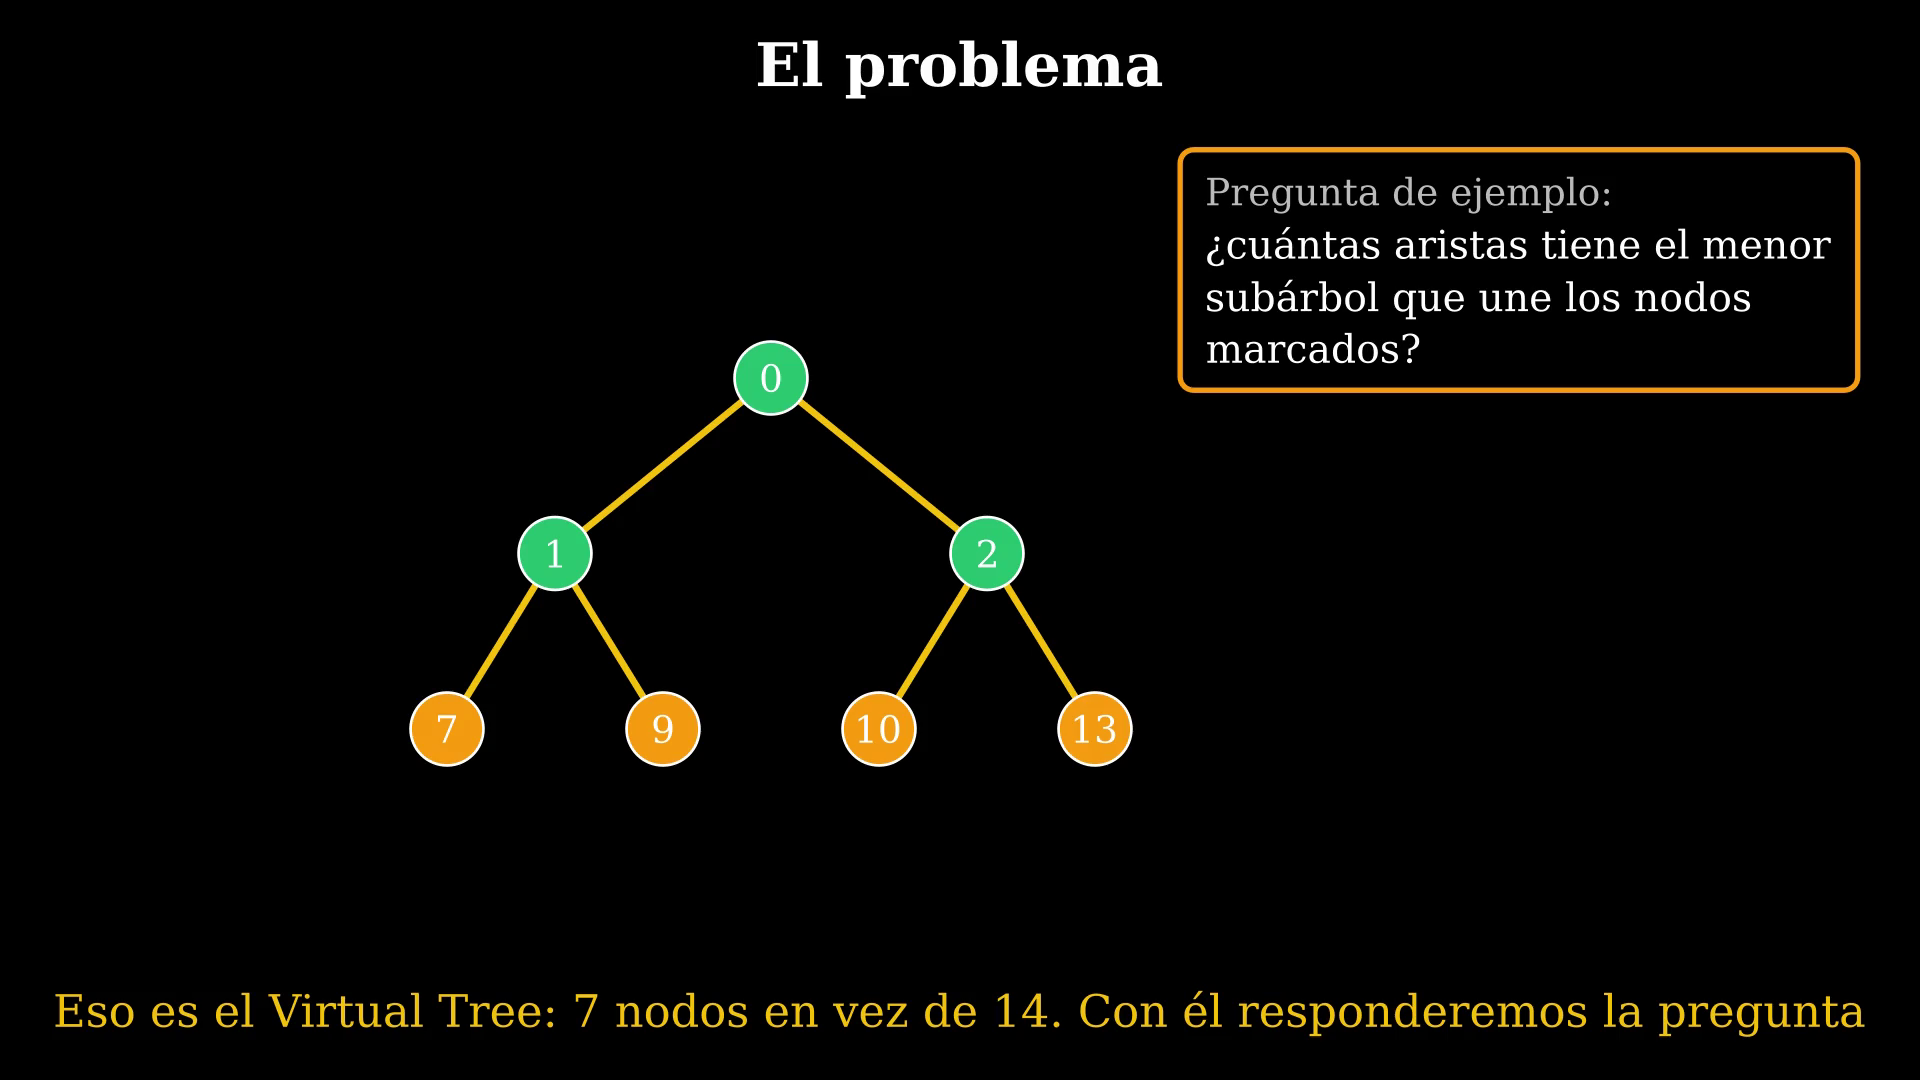
\includegraphics[width=\textwidth]{figuras/01_problema.png}
    \caption{El problema: pregunta concreta y el árbol comprimido como meta.}
  \end{subfigure}\hfill
  \begin{subfigure}[t]{0.49\textwidth}
    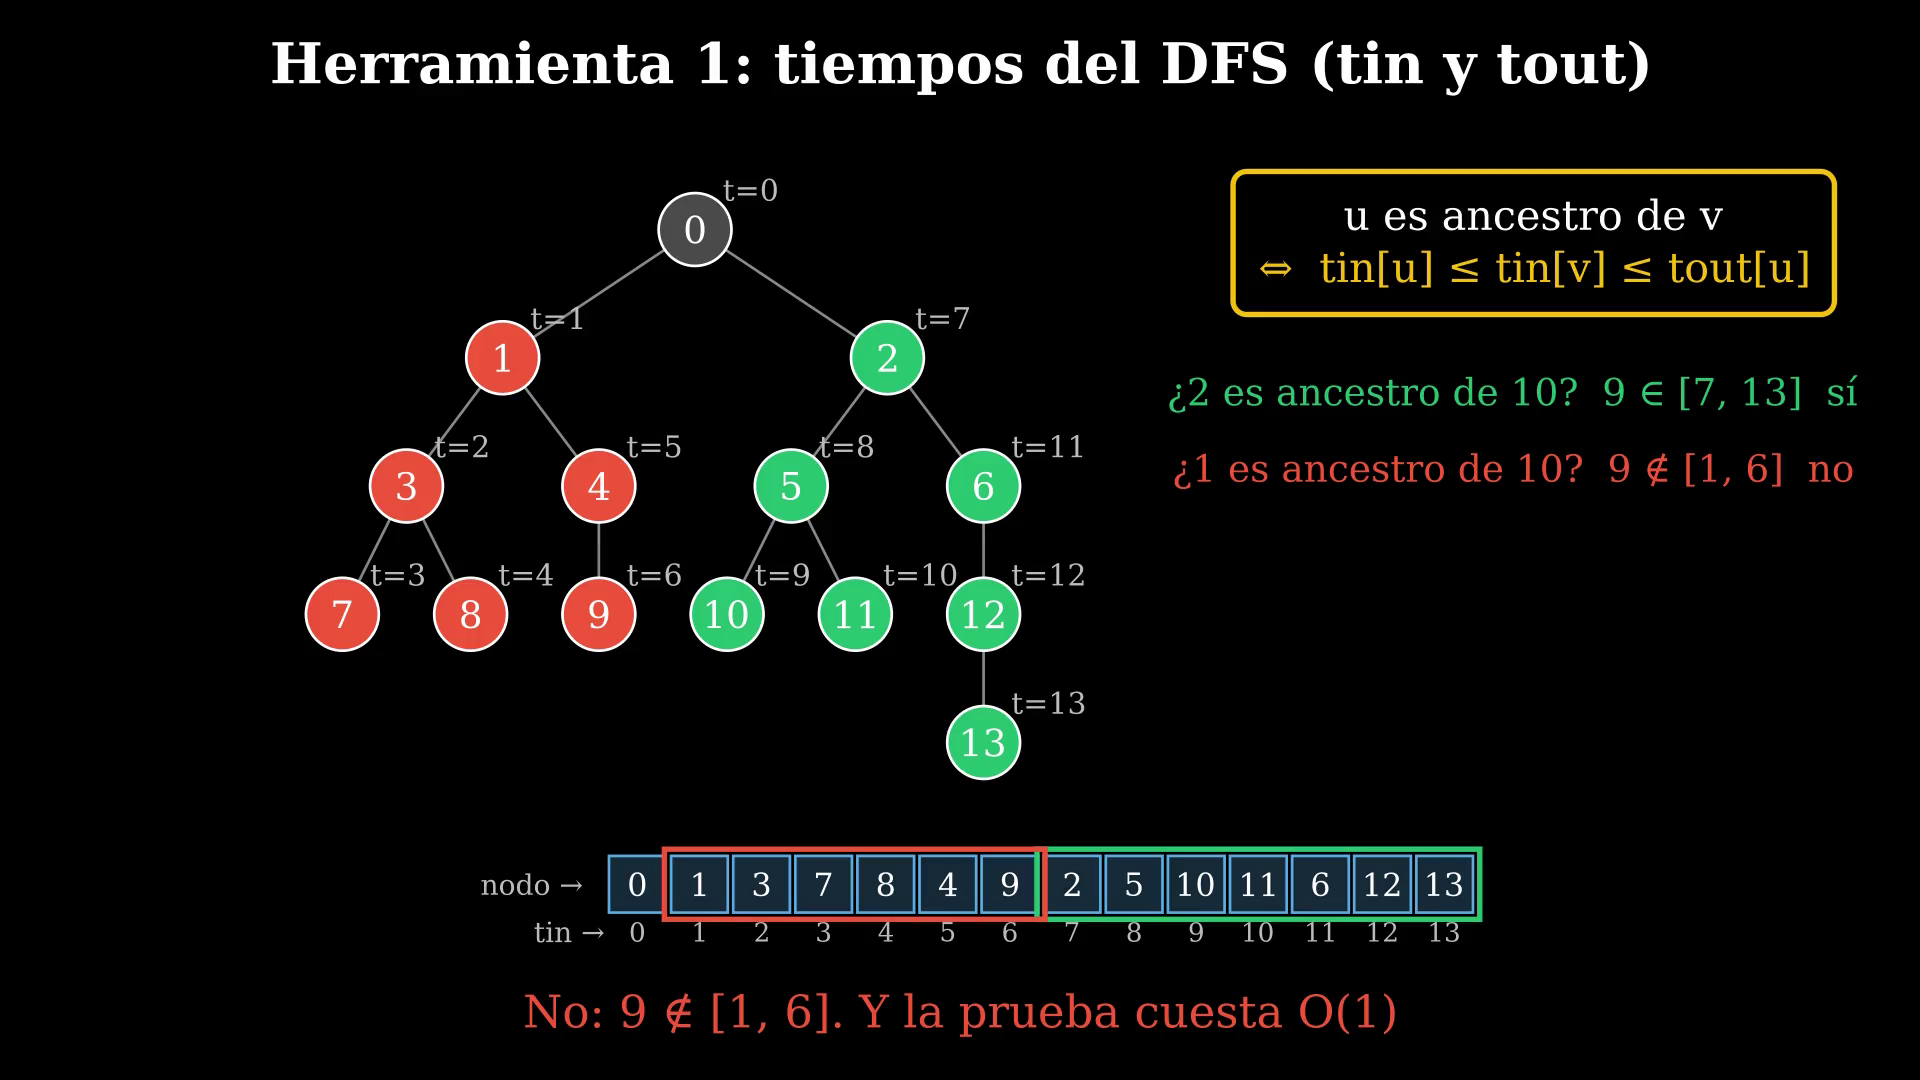
\includegraphics[width=\textwidth]{figuras/02_tin.png}
    \caption{Herramienta 1: subárboles como bloques de \texttt{tin} y pregunta rápida al espectador.}
  \end{subfigure}

  \vspace{0.25cm}
  \begin{subfigure}[t]{0.49\textwidth}
    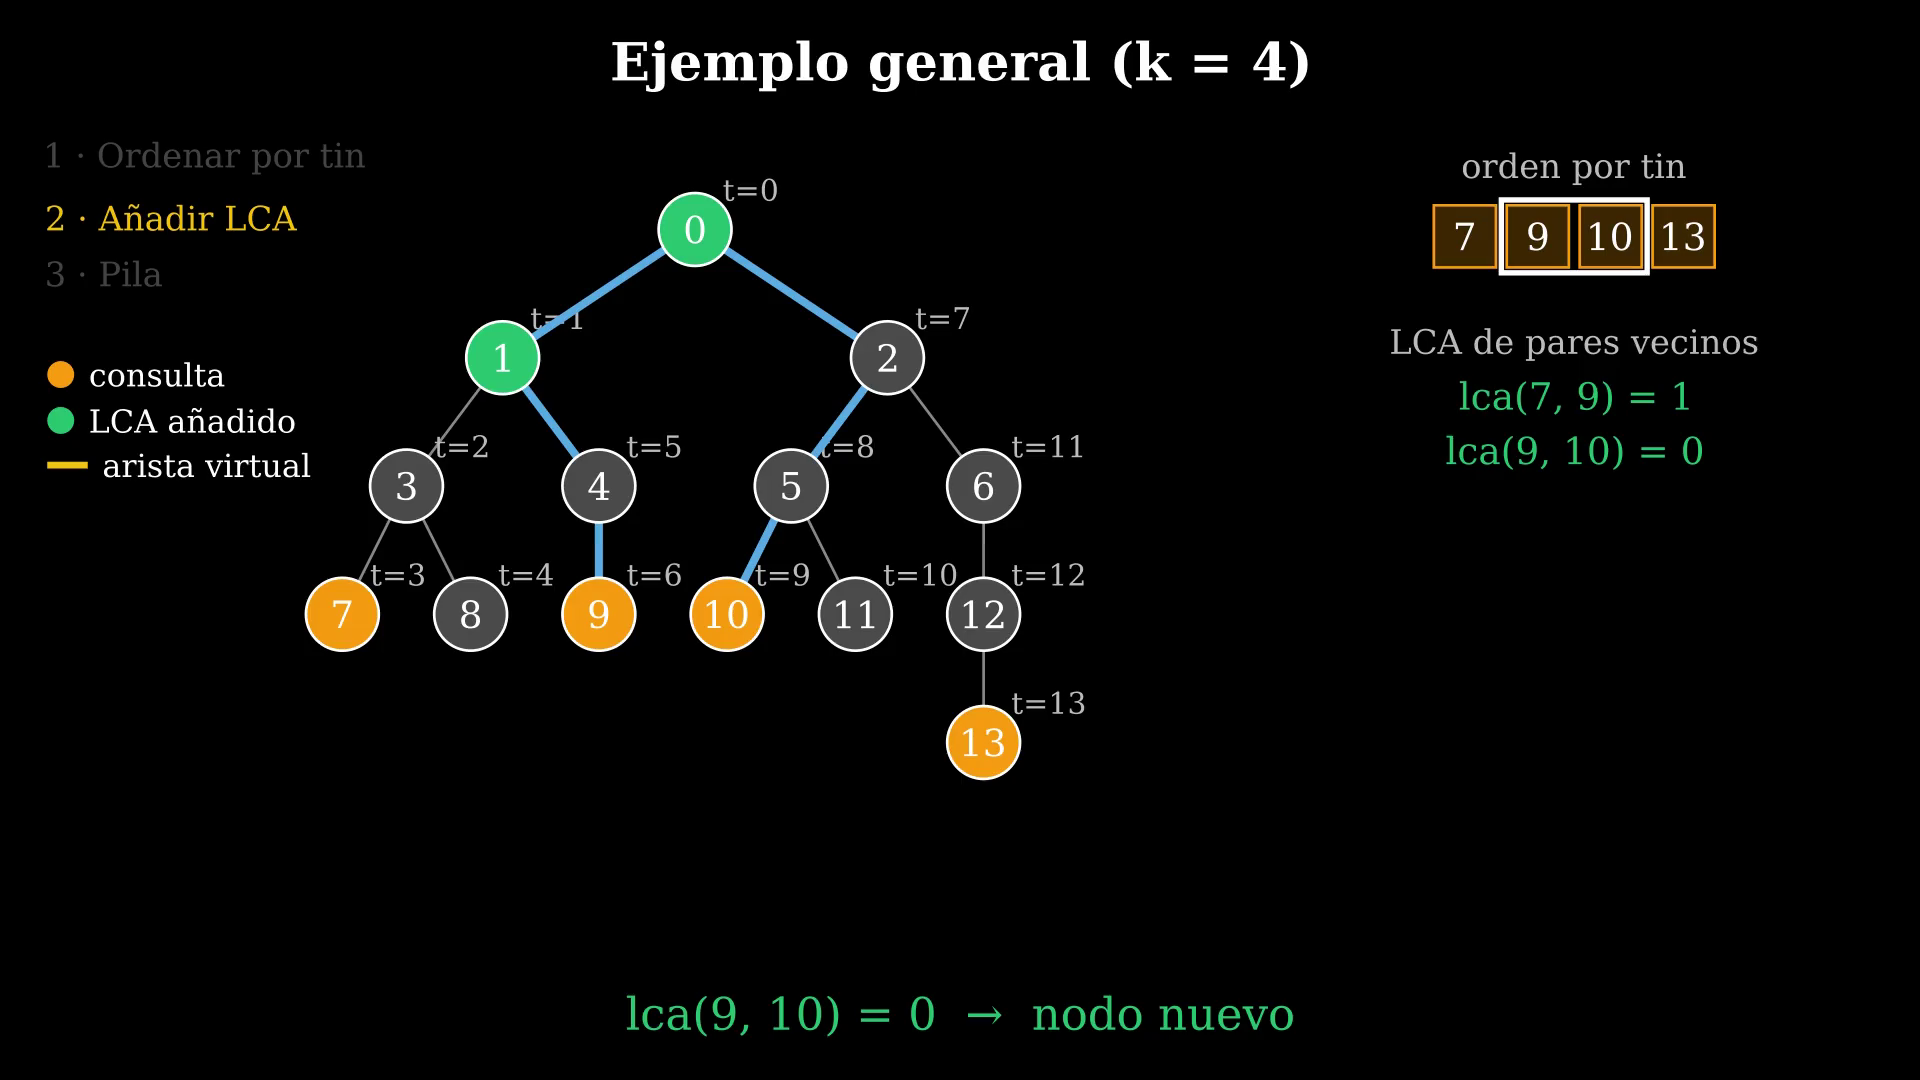
\includegraphics[width=\textwidth]{figuras/03_lca.png}
    \caption{Paso 2: camino de cada par vecino hasta su LCA; a la izquierda, paso actual y leyenda.}
  \end{subfigure}\hfill
  \begin{subfigure}[t]{0.49\textwidth}
    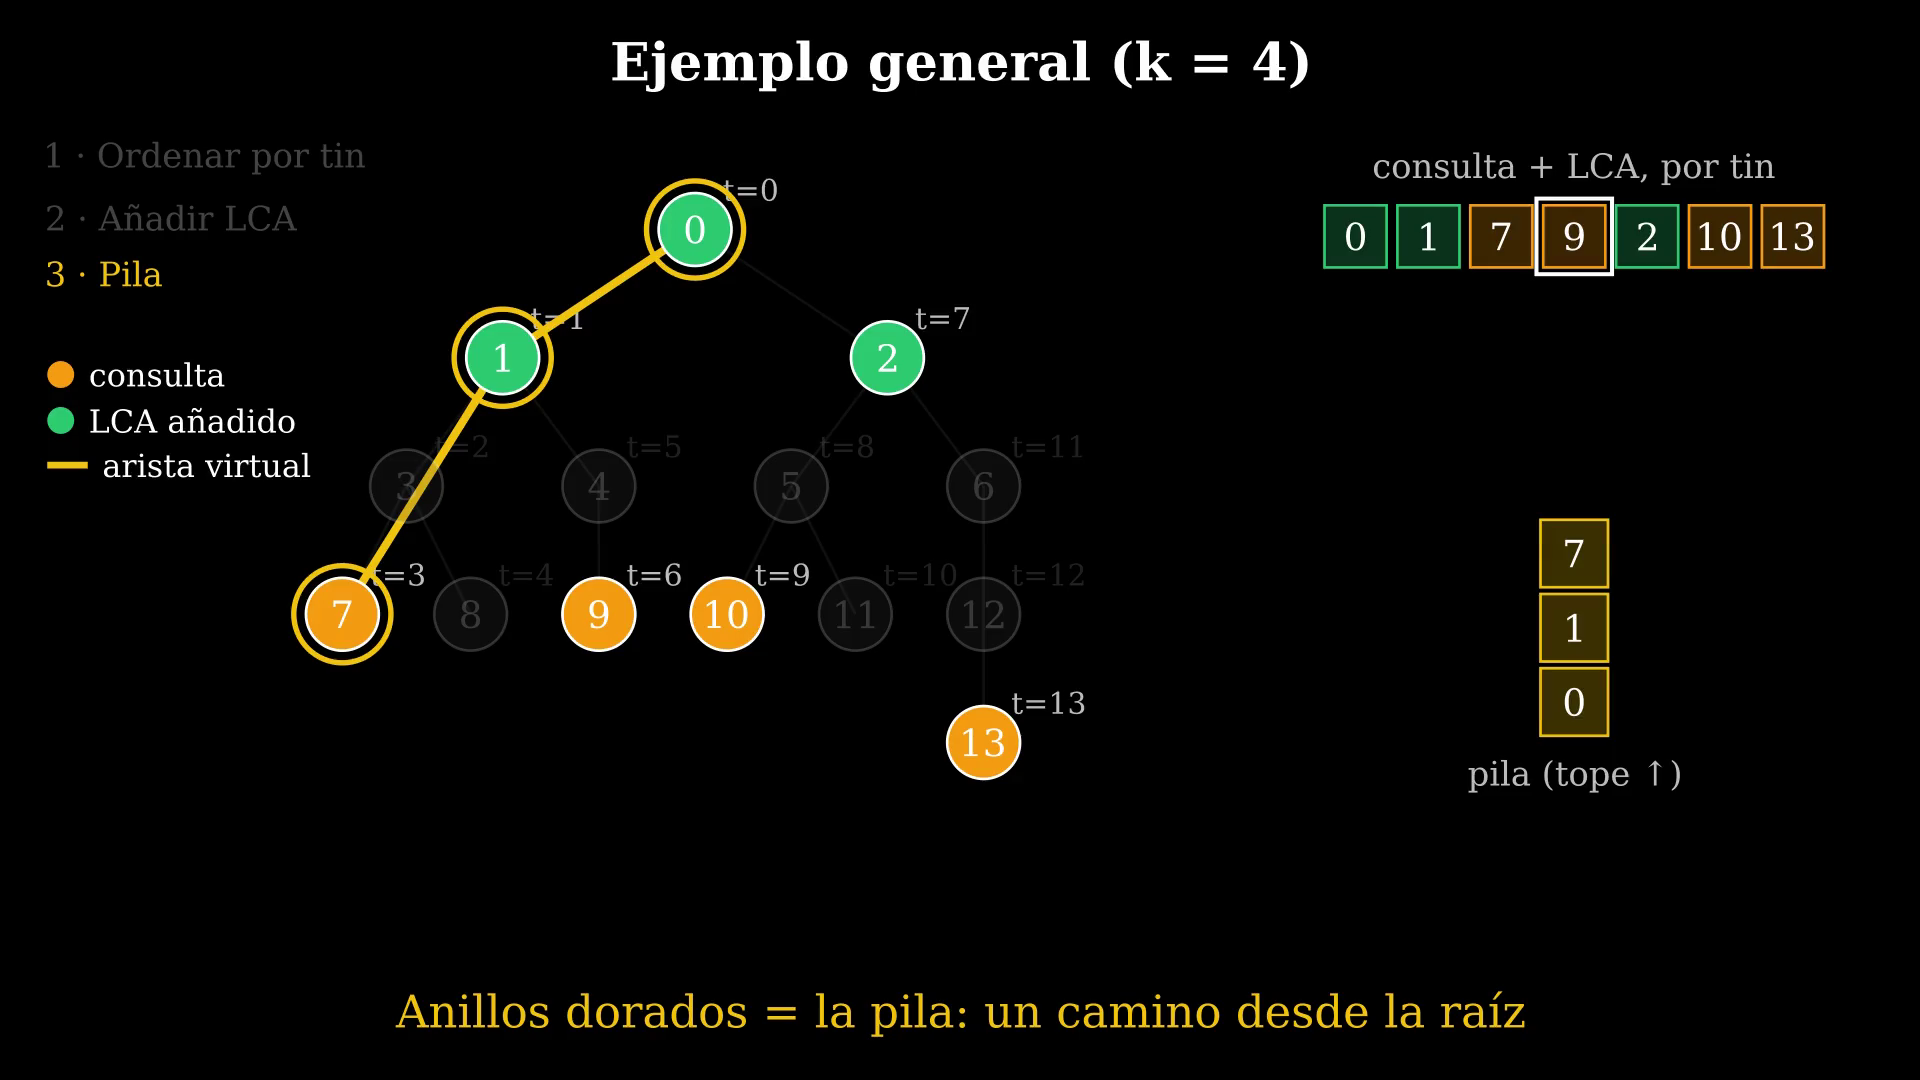
\includegraphics[width=\textwidth]{figuras/04_pila.png}
    \caption{Paso 3: los anillos dorados muestran la pila como un camino desde la raíz.}
  \end{subfigure}

  \vspace{0.25cm}
  \begin{subfigure}[t]{0.49\textwidth}
    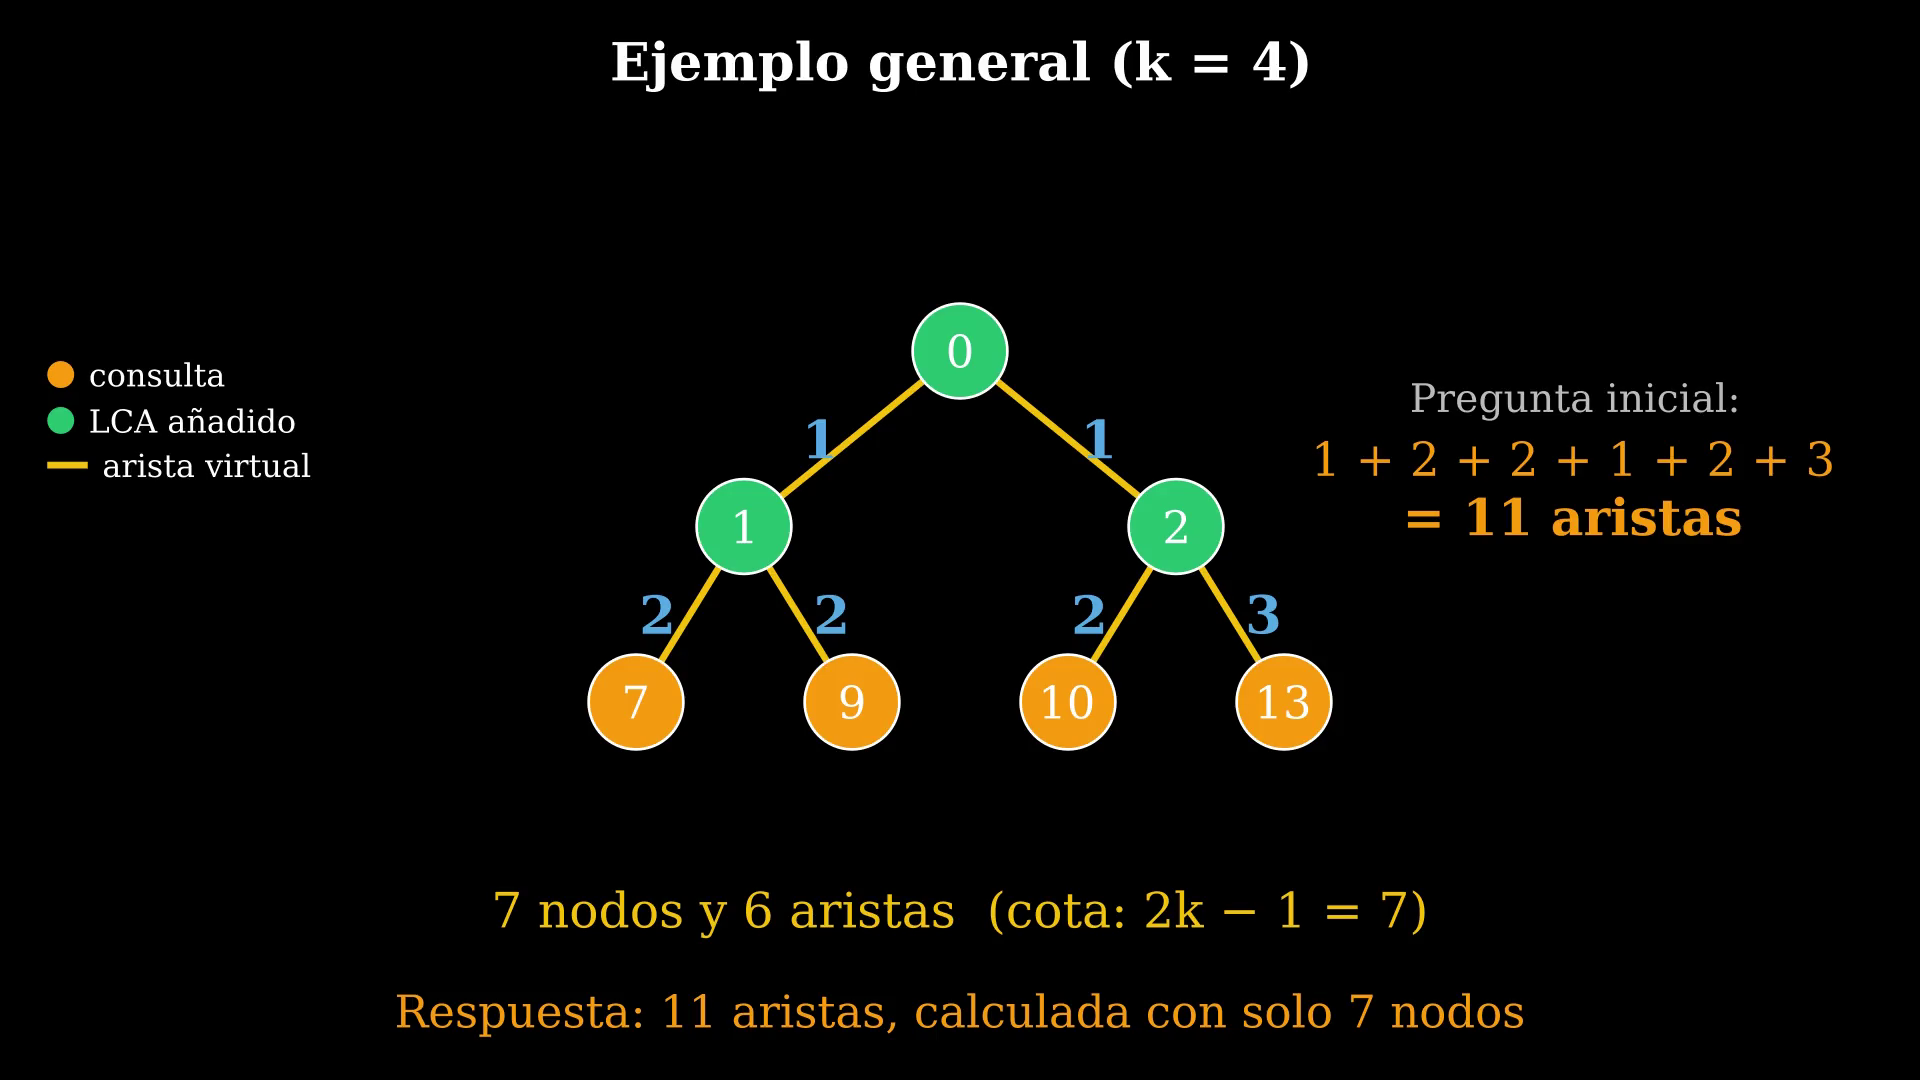
\includegraphics[width=\textwidth]{figuras/05_respuesta.png}
    \caption{Resultado: la pregunta inicial se responde sumando las aristas virtuales (11).}
  \end{subfigure}\hfill
  \begin{subfigure}[t]{0.49\textwidth}
    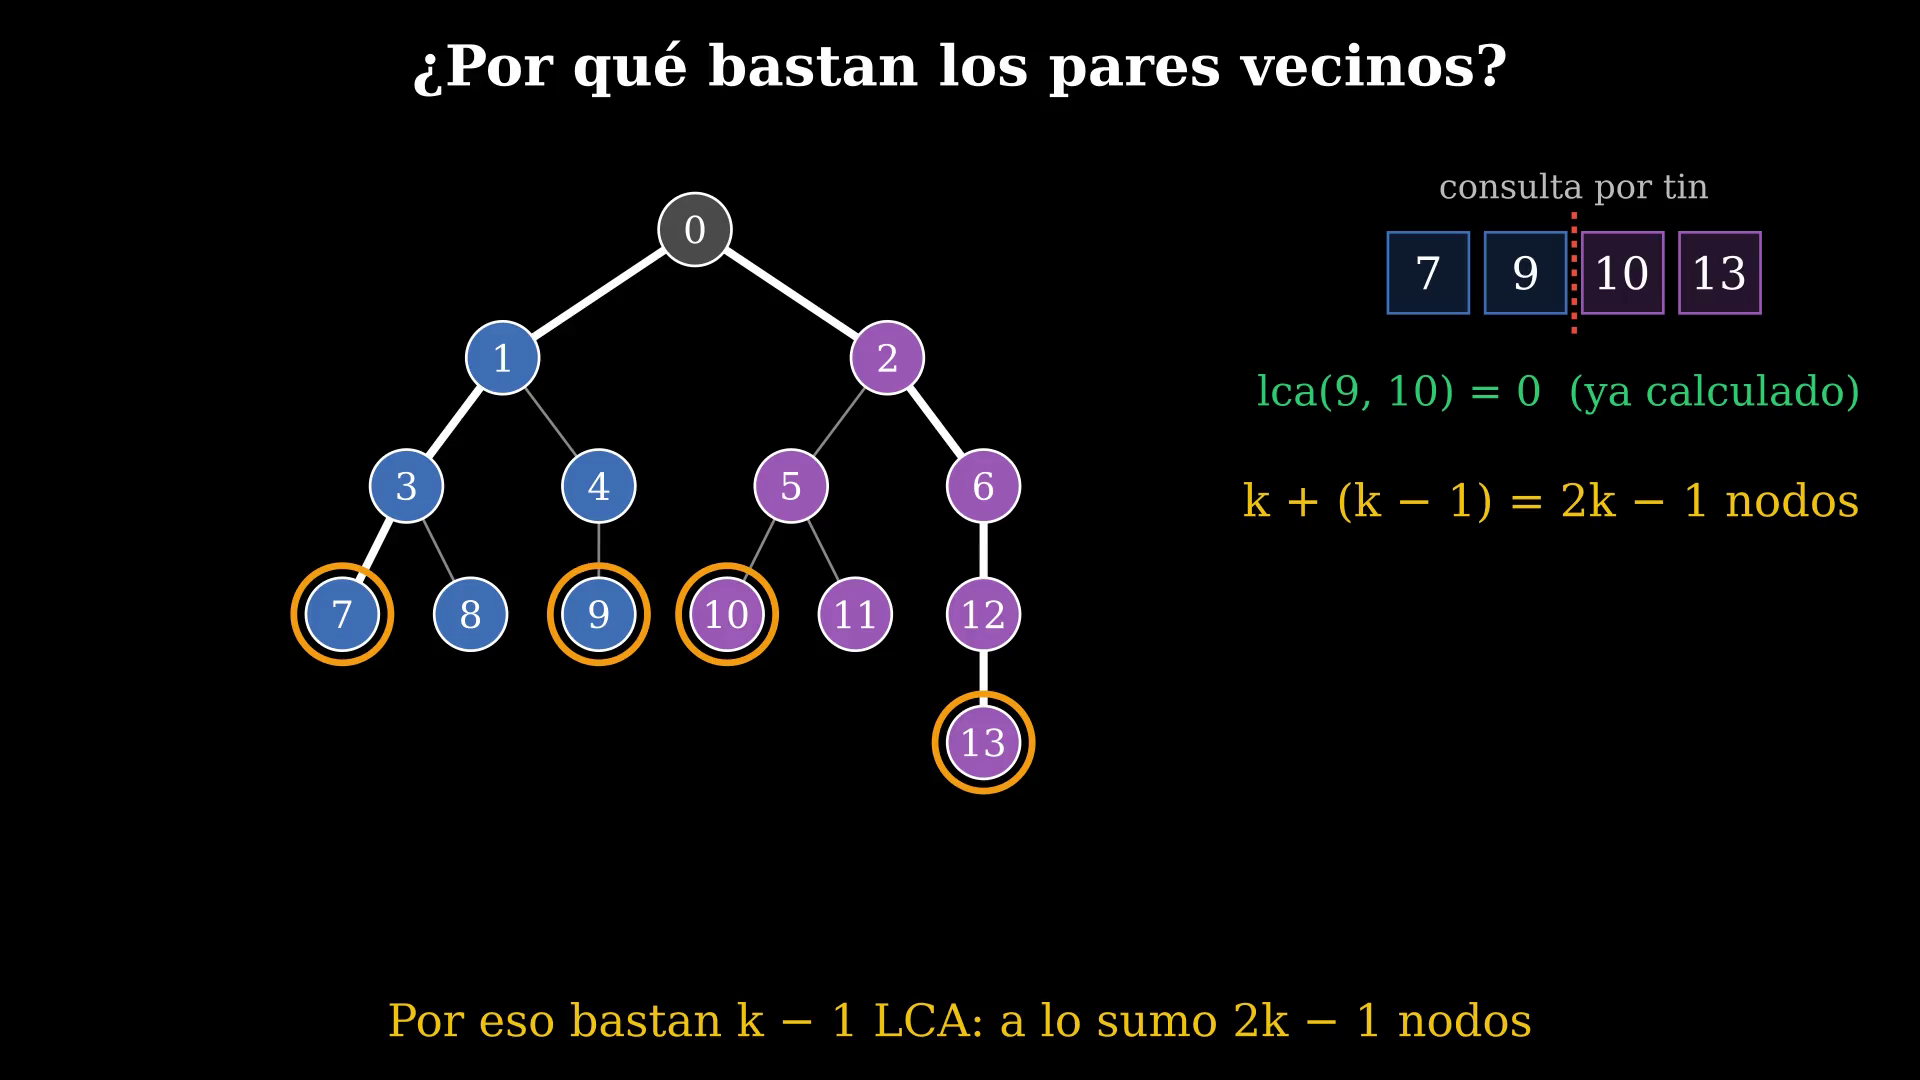
\includegraphics[width=\textwidth]{figuras/06_porque.png}
    \caption{¿Por qué bastan los pares vecinos? El color cambia una sola vez, entre 9 y 10.}
  \end{subfigure}

  \vspace{0.25cm}
  \begin{subfigure}[t]{0.49\textwidth}
    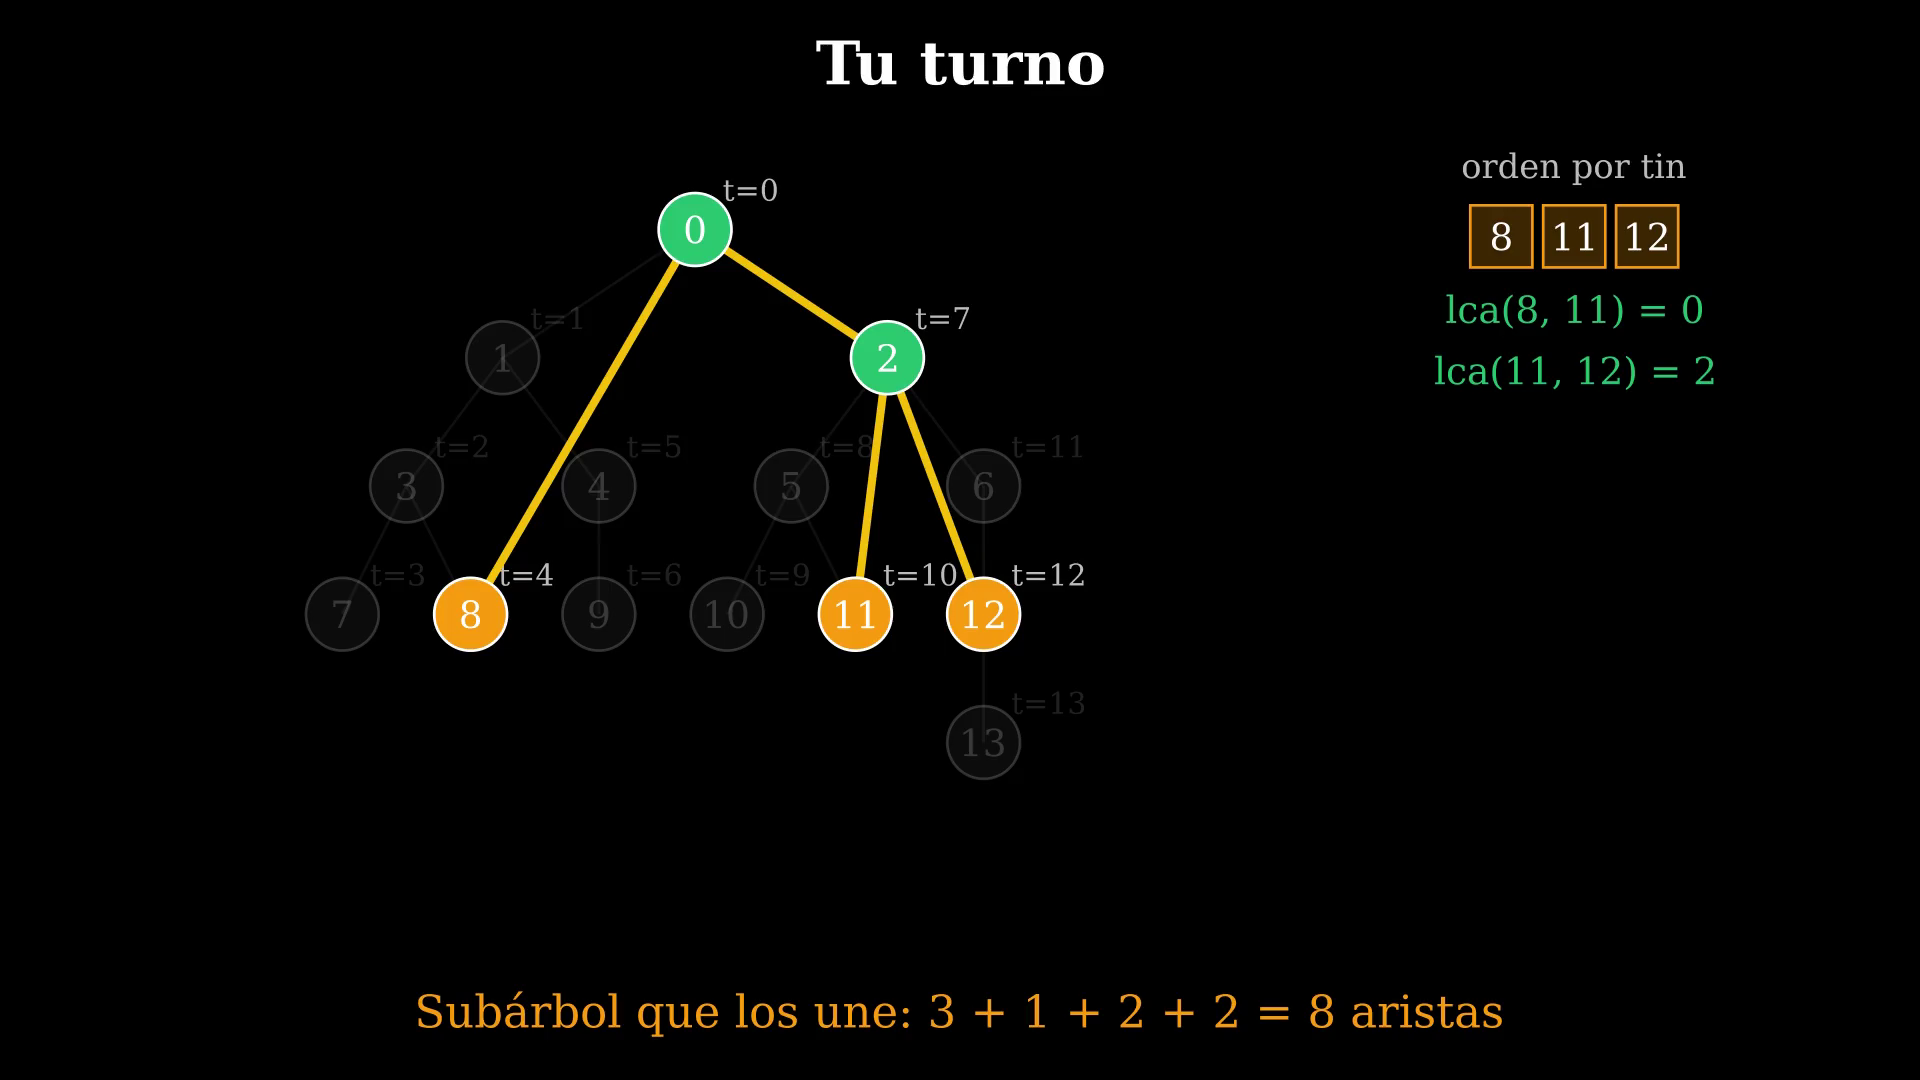
\includegraphics[width=\textwidth]{figuras/07_ejercicio.png}
    \caption{Tu turno: solución del ejercicio (5 nodos $= 2k-1$).}
  \end{subfigure}\hfill
  \begin{subfigure}[t]{0.49\textwidth}
    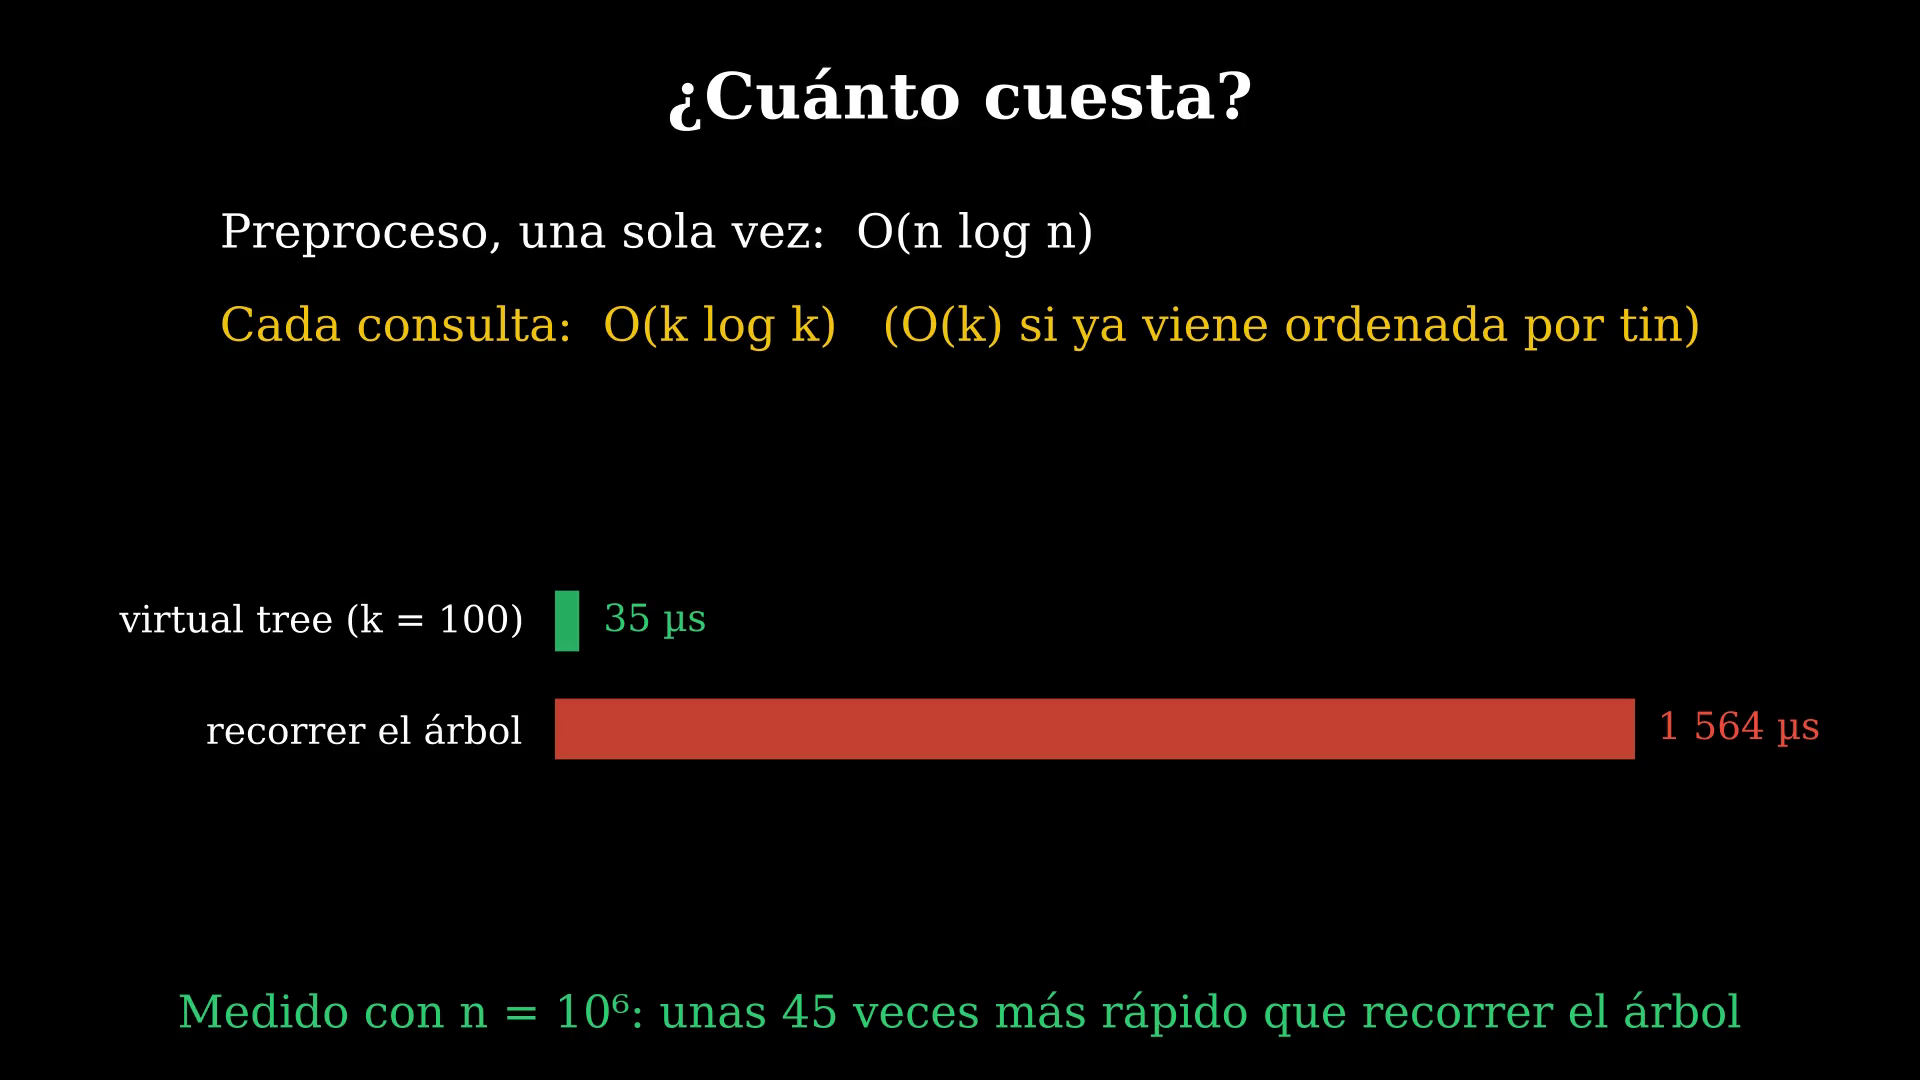
\includegraphics[width=\textwidth]{figuras/08_costo.png}
    \caption{Costo medido: virtual tree frente a recorrer todo el árbol ($n=10^6$).}
  \end{subfigure}
  \caption{Capturas del video.}
\end{figure}

% ======================= 7. CONCLUSIONES =======================
\section{Conclusiones}

\begin{enumerate}[label=\arabic*.]
  \item El virtual tree desacopla el costo de una consulta del tamaño del árbol: tras un
        preprocesamiento $O(n \log n)$, cada consulta de $k$ nodos se resuelve en
        $O(k \log k)$ (u $O(k)$ si la entrada ya está ordenada) y produce un árbol de a lo
        sumo $2k-1$ nodos. Las mediciones lo confirman: con $k$ fijo, el tiempo casi no
        cambia al pasar de $10^3$ a $10^6$ nodos.
  \item El orden de entrada del DFS es la pieza clave del algoritmo: como cada subárbol ocupa
        un intervalo contiguo de \texttt{tin}, basta revisar los LCA de pares adyacentes para
        obtener todos los puntos de ramificación, y una pila resuelve las relaciones de
        ancestro en tiempo lineal.
  \item Evitar la segunda ordenación (variante $O(k)$) reduce el tiempo entre 1.5 y 5.7 veces
        en la práctica, lo que importa cuando la suma de los $k$ es grande.
  \item Generar la animación a partir de una traza producida por la propia implementación
        en C++ evita inconsistencias entre lo que se explica y lo que el código hace, y las
        pruebas contra fuerza bruta validaron también los casos borde, incluido un árbol de
        $10^6$ nodos de profundidad.
\end{enumerate}

% ======================= REFERENCIAS =======================
\section*{Referencias}
\addcontentsline{toc}{section}{Referencias}
\begin{itemize}
  \item M.~A. Bender y M.~Farach-Colton. \emph{The LCA Problem Revisited}. LATIN 2000,
        LNCS 1776, pp.~88--94. (Reducción de LCA a RMQ sobre el recorrido de Euler.)
  \item CP-Algorithms. \emph{Lowest Common Ancestor} (reducción a RMQ con el recorrido de
        Euler). \url{https://cp-algorithms.com/graph/lca.html}.
  \item Codeforces, problema 613D \emph{Kingdom and Its Cities} (aplicación típica del
        virtual tree). \url{https://codeforces.com/problemset/problem/613/D}.
  \item Documentación de Manim Community. \url{https://docs.manim.community}.
\end{itemize}

\end{document}
